\chapter{Background \label{sec:background}}
\todo[inline]{Background: this should include all (appropriately cited) information (concepts and prior literature) for a layperson to understand your project/experiment. \\ - NEED TO RESEARCH AND DISCUSS THE EFFECTS OF NOISE AND TYPICAL ATTNENUATION}

\noindent
This chapter collates the necessary background information for the project, including the fundamentals of passive radar, the use of illuminators of opportunity, range doppler mapping, radio hardware, digital signal processing, IoT architecture, and networking with embedded hardware.


\section{Passive Radar Fundamentals}
The key and unique feature of passive radar is its utilisation of existing illuminators of opportunity, such as television or radio broadcasts, to detect and track objects. The technology has been around since the early 20th century, with modern interest accelerated due to the use of passive radar systems on UHF TV signals and VHF FM radio tranmission systems in the 1980's \cite{FundamentalsPassiveRadar}. Equivalent terms used to describe passive radar include passive coherent location (PCL), and passive covert radar (PCR), parasitic radar, piggyback radar. Specifically, \textit{bistatic} radar refers to the distributed design of the transmitter and receiver, as opposed to classic \textit{monostatic} radar. As reflectd by Figure \ref{fig: topology} below, the turning parabolic of monostatic radar is able to receive both range and bearing of the signal echo, whereas passive bistatic radar measures time delay of the echos from the target, allowing doppler shift from the relative speed of the target to be measured.

\begin{figure}[htbp]
    \centering
    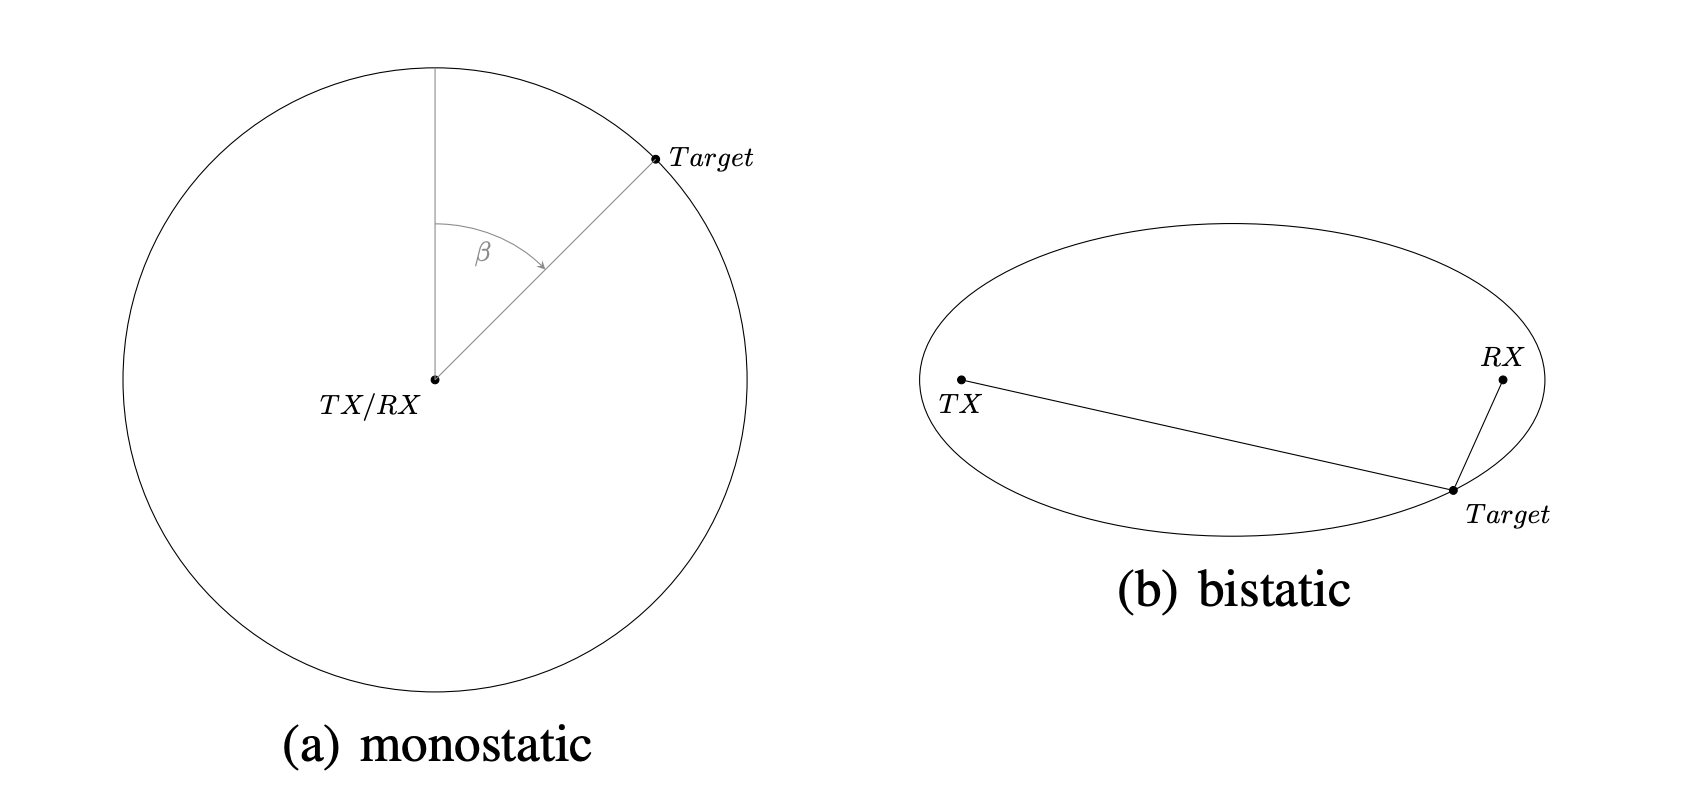
\includegraphics[width=0.8\textwidth]{monoBi.jpg}
    \caption{Monostatic (a) and bistatic (b) radar topologies \cite{IOTpassiveRadar}}
    \label{fig: topology}
\end{figure}

\par 
\vspace{0.5cm} 
\noindent The geometry of passive bistatic radar can be further explored and equations can be mapped accordingly, with the distance between the transmitter and receiver \textit{R} being determined by known quantities such as the baseline as reflected below in Figure \ref{fig:geometry}.


\par \vspace{0.5cm} 
\noindent The bistatic range \( R_R \) is given by:
\begin{equation}
R_R = \frac{(R_T + R_R)^2 - L^2}{2(R_T + R_R + L \sin \theta_R)}
\end{equation}

\noindent The Doppler shift \( f_D \) is given by the rate of change of the bistatic range sum:
\begin{equation}
f_D = \frac{1}{\lambda} \frac{d}{dt}(R_T + R_R) \xrightarrow{} f_D = \frac{2v}{\lambda} \cos \delta \cos(\frac{\beta}{2})
\end{equation}
In the case of this project, both the TX (illuminator of opportunity) and the RX (embedded passive detection system) will be static, and the target will be moving, simplifying the mathematical calculations as much as possible, resulting in the cos version of equation 2 above. 

\par
The Doppler shift will be used to determine the speed of the target as well as its relative directional motion, and the range will be used to determine the distance of the target from the receiver. Another important feature of bistatic passive radar systems is its performance which can be equated through the bistatic radar equation, which is equivalently derived as the monostatic radar equation \cite{FundamentalsPassiveRadar}. 
\vspace{0.5cm} 
\begin{equation}
    \frac{P_r}{P_n} = \frac{P_t G_t}{4\pi R_T^2} \cdot \sigma_B \cdot \frac{1}{4\pi R_R^2} \cdot \frac{G_r \lambda^2}{4\pi} \cdot \frac{1}{k T_0 B F}
\end{equation}
Where:
\begin{multicols}{2}
    \begin{itemize}
    \item \( P_r \) is the received target echo power.
    \item \( P_n \) is the receiver noise power.
    \item \( P_t \) is the transmit power.
    \item \( G_t \) is the transmit antenna gain.
    \item \( R_T \) is the transmitter-to-target range.
    \item \( \sigma_B \) is the target bistatic radar cross section.
    \item \( R_R \) is the target-to-receiver range.
    \item \( G_r \) is the receive antenna gain.
    \item \( \lambda \) is the signal wavelength.
    \item \( k \) is Boltzmann’s constant (\( 1.38 \times 10^{-23} \) JK\(^{-1}\)).
    \item \( T_0 \) is the noise reference temperature.
    \item \( B \) is the receiver effective bandwidth.
    \item \( F \) is the receiver effective noise figure.
    \end{itemize}
\end{multicols}

\begin{figure}[htbp]
    \centering
    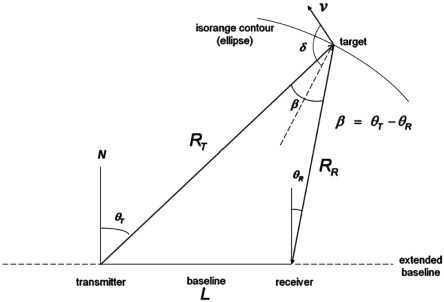
\includegraphics[width=0.8\textwidth]{geomPR.jpg}
    \caption{Bistatic radar geometry \cite{FundamentalsPassiveRadar}}
    \label{fig:geometry}
\end{figure}

\par \vspace{0.5cm}
\noindent The denominator of the bistatic radar equation includes the term \( \frac{1}{R_T^2 R_R^2} \).This term implies that with omnidirectional antenna patterns, the contours of constant signal-to-noise ratio (SNR) are described by the equation \( R_T R_R = \text{constant} \), which represents Ovals of Cassini. These ovals represent the locations in a given PBR co-ordinate sytem where the distances from the target to the transmitter and receiver remain the same. In the case of directional antennas, these contours are altered. Moreover, the signal-to-noise ratio is minimized when the target is equidistant from the transmitter and receiver (\( R_T = R_R \)), and maximized when the target is closer to either the transmitter or receiver \cite{FundamentalsPassiveRadar}.

\par \vspace{0.5cm} 
\todo[inline]{NEED TO MENTION / RESEARCH THE EFFECT OF NOISE AND DECIBELS EXPECTED HERE.}
% \noindent Ideally this project would process just the target signal, however, that is an unrealistic expectation due to the presence of clutter. Clutter refers to unwanted signal that eminates from objects in the natural environment such as buildings, trees and ground \cite{zhang2023intelligent}. This process of target signal clutter suppression and its impact on range doppler mapping will be discussed later in the literature review.  

\section{Illuminators of Opportunity}
The illuminator of opportunity is the signal that is used to illuminate the target, and is the primary source of the signal that is received by the passive radar system. The illuminator of opportunity can be any signal that is transmitted through the air, such as television or radio broadcasts, and can be tailored to the specific requirements of the passive radar system. Griffiths and Baker outline the three key paramaters when selecting an illuminator \cite{INTRO2017}:
\begin{enumerate}[label=\arabic*.]
    \item The \textbf{Power Density} at the target: It refers to the strength of the signal (in Watts per square meter) that reaches the target area from the illuminator. Higher power density can improve detection performance due to a stronger return signal.
    \item The \textbf{Nature of the Waveform}: This includes the waveform's properties, such as bandwidth and modulation, which can affect the radar's resolution and ability to distinguish between targets and clutter.
    \item The \textbf{Coverage}: The spatial area over which the illuminator's signal is spread. Adequate coverage is essential to ensure the target is within the illuminator's effective range.
\end{enumerate}

Illuminator signals are not limited to terrestrial signals, and can also include signals from satellites, and can be tailored to the specific requirements of the passive radar system. The illuminator of opportunity primarily explored for this project is the DAB+ signal, and the target signal will be aerial vehicles - most likely in the form of civillian passenger jets. The DAB+ signal is a good option due to its high power density, and its relatively high bandwidth, which can be used to improve the radar's resolution and ability to distinguish between targets and clutter. Moreover, the geographical proximity of a DAB+ transmitter at Mt Cootha to the University of Queensland, St Lucia campus, making it a potentially ideal choice for the project. Another prospective digital illuminator signal is DVB-T (digital video broadcast - terrestrial), which is similar in its digital modulation to DAB, but provides increased bandwidth and signal power \cite{DVBsignal}. Furthemore, as shown by Yin et. al \cite{DVBnoise}, due to the relative complexity of  DVB visual signals, more signal processing steps can be required, which could exceed prospective hardware limitations of this project.

\par \vspace{0.5cm} 
\noindent A potential problem associated with the use of DAB as an illuminator is direct signal interference (DSI), with the effects being amplified in urban environments. Coleman et. al \cite{DABfeatures} explain that the sheer signal size of direct illuminator size relative to surveillance signal size results in a high level of DSI. They outline that the cross polarisation of the transmitted DAB signal can be utilised along with illuminator cancellation filtering to attain higher level suppression. The leakage of the illuminator signal into the target signal can be due to a range of factors including buildings, trees and other reflective items as highlighted by Palmer et. al \cite{DTSO2009}.

\par \vspace{0.5cm} 
\noindent Typical characteristics of Australian DAB+ signals include frequency of just over 200MHz, bandwidth of approximately 1.5MHz, and a minimal output power of 10kW effective radiated power (ERP), consequently covering a large area \cite{DABfeatures}. These digital signals employ a modulation scheme called COFDM (coded orthogonal frequency division multiplexing), which is a form of multi-carrier modulation that is robust against multipath interference \cite{INTRO2017}. COFDM works by dividing the signal into multiple, simultaneous streams which are orthogonal to each other, modulated at a different frequency, maximising robust signal propogation. This is particularly useful in the context of passive radar, as it allows for the target and reference signal to be received by the passive radar system even if it has been reflected off multiple surfaces, such as buildings or trees.

\todo[inline]{FM / other signals: why / why not?}

\par \vspace{0.5cm} 
\noindent All of the above features result in DAB signals being condusive for ambiguity function performance (analyzed in further detail below). This can mainly be attributed to the relatively wide bandwidth of DAB enabling good resolution, constant DAB envelope stemming from COFDM protocol, and the multipath resistance \cite{DABambiguity}.




\section{Range Doppler Mapping}
Range doppler mapping is a technique used to determine the distance and relative velocity of targets by analyzing the frequency shift (Doppler shift) and time delay of the received signals after they are reflected off the targets. The signal response of a target at a particular range and velocity can be predicted by the ambiguity function seen in equation \ref*{eq:ambiguity} \cite{INTRO2017}. 
\begin{equation}
    \chi(\tau, f) = \int s_{\text{reference}}(t) s_{\text{received}}^*(t - \tau) e^{j2\pi f t} \, dt \label{eq:ambiguity}
\end{equation}

Where:
\begin{multicols}{2}
\begin{itemize}
\item \( \chi(\tau, f) \) is the ambiguity function.
\item \( \tau \) is the time delay.
\item \( f \) is the Doppler frequency.
\item \( s_1(t) \) is the transmitted signal.
\item \( s_2(t) \) is the received signal.
\item \( s_2^*(t - \tau) \) is the complex conjugate of the received signal, time-shifted by \( \tau \).
\item \( e^{j2\pi f t} \) is the complex exponential representing the Doppler shift.
\item The integral is taken over all time \( t \).
\end{itemize}
\end{multicols}

\noindent The ambiguity function can be plotted, thereby visualising resolution, sidelobe patterns and any discrepancies in range and doppler. This is especially important for passive bistatic radar, whereby waveforms are not explicitly designed for radar and the geometry also has an impact \cite{FundamentalsPassiveRadar}. Hughes visualises the geometry considerations and potential flaws of generic passive bistatic configuration below in Figure \ref{fig:ambiguity}.

\begin{figure}[htbp]
    \centering
    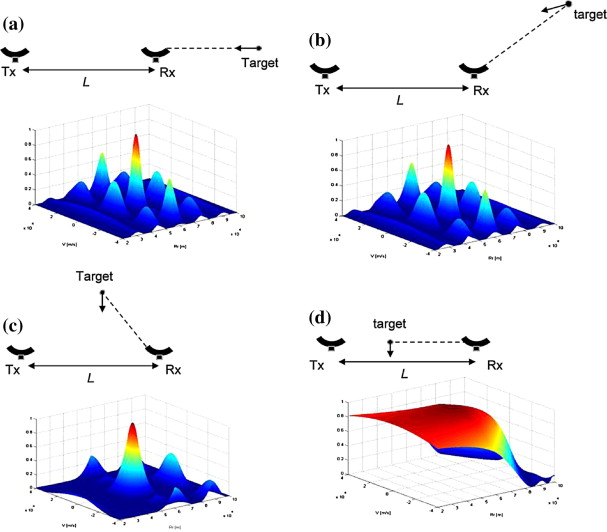
\includegraphics[width=0.7\textwidth]{ambiguity.jpg}
    \caption{Geometry and ambiguity function \cite{FundamentalsPassiveRadar}}
    \label{fig:ambiguity}
\end{figure}

\par \vspace{0.5cm} 
\noindent Understanding the link between geometric configuration and theoretical signal properties, the practical manifestation of the ambiguity function is range doppler mapping. As shown in Figure \ref{fig:rangeDoppler}, the map is a heat map and is derived with filters for noise minimsation, allowing for the visualisation of the target signal with minimal clutter. 

\begin{figure}[htbp]
    \centering
    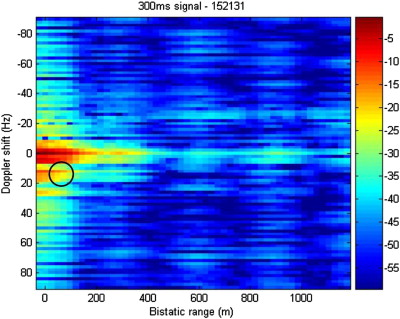
\includegraphics[width=0.6\textwidth]{rangeDoppler.jpg}
    \caption{Example of range doppler map for WiFi PBR \cite{FundamentalsPassiveRadar}}
    \label{fig:rangeDoppler}
\end{figure}

\todo[inline]{Should i use a better RDM??}
\par  
\noindent In the case of this project, the time delay will be utilised to calculate the bistatic range (x axis) and the Doppler shift will be used to calculate the relative velocity of the target (y axis). In summary, ambiguity function and subequent range doppler mapping will be vital for mapping the DAB+ signal characteristics for given geometry and motion of the surveilled target. \todo{MORE DETAIL}



\section{Radio Hardware}
Given the low cost aims of this project, hardware cost and performance is a major consideration. Luckily, the proliferation of Software Defined Radio (SDR) has enabled low cost hardware modules enabling easy access to radio frequency (RF) signals \cite{SDRtheory}.

\todo[inline]{More specifics about SDR}

\par \vspace{0.5cm}
The most popular and lowest cost SDR module is the RTL-SDR, which is a USB dongle that can be used to receive and decode a wide range of RF signals. The RTL-SDR is based on the Realtek RTL2832U chipset, and has a frequency range of 24MHz to 1.7GHz, and a bandwidth of 3.2MHz. The RTL-SDR is also relatively cheap, with a price of around \$40 AUD. Moreover, the RTL-SDR is compatible with a wide range of software, including MATLAB, and GNU radio \cite{SDRdongle}. Given the digital nature of the DAB+ signal, the direct reference signal and the target surveillance signal can in theory be sampled by a singular RTL2832U module as shown by Barrot et.al \cite{DABsingleRadar}.

\todo[inline]{Block diagram of SDR transceiver?}

\par \vspace{0.5cm}
There are also a range of other off the shelf SDR options such as BladeRF and LimeSDR, which provide marginally improved performance at a substantial increase in cost and hardware \cite{SDRhardware}.  Regardless of sampling hardware architecture, based on previous studies and the nature of the DAB+ signal and modulation framework, a sampling rate of 2.048\,MS/s is prudent \cite{IOTpassiveRadar}. This hardware can be scaled up, accordingly providing a reference antenna and a surveillance antenna, as seen in Yardleys 2007 DAB receiver project \cite{antennaArchitecture}. On the contrary, as a potential extension, the use of a single antenna can be attempted with additional reconstruction processing required (providing lower hardware cost), this has been achieved by Barott and Engle \cite{DABsingleRadar}.


\section{Digital Signal Processing}
Broadly, the goal of the signal processing for general passive bistatic radar is to extract a range doppler map from a received signal. Obtaining a range doppler map involves a few steps, with specifics depending on the IOO chosen along with number of sampling channels. Furthermore, there is the option of autocorrelating these signals via correlation integrals which is the most time and compute intense, or through Batches algorithm in the frequency domain \todo{batches citation needed}. Prior to the advent of of digital broadcasts, analague broadcast processing involved comprehensive filtering and synchronisation of at least two input channels\cite{DSPfm}. However, more recently, given the nature of DAB / DVB-T and its COFDM modulation, filtering and synchronisation can be replaced with reconstruction of the surveillance signal \cite{DSPdab}, replacing the need for dual channel configuration. The use of a singular antenna / channel setup is affirmed by Barott et. al \cite{DABsingleRadar} who utilised DAB passive radar to track micro-UAVs.

\begin{wrapfigure}{r}{0.6\textwidth} % This places the figure on the right and occupies 60% of the text width
    \centering
    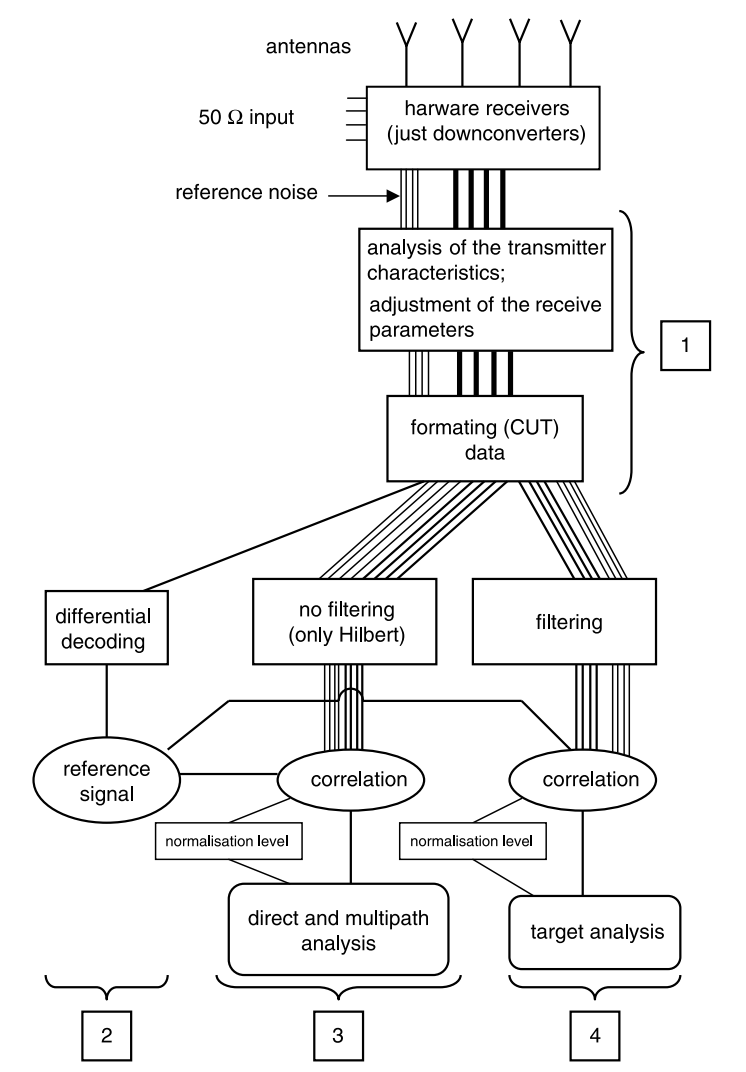
\includegraphics[width=0.45\textwidth]{DSPprocess.png}
    \caption{Main steps of signal processing \cite{detectionDABmodulation}}
    \label{fig:DSP}
\end{wrapfigure}


\par \vspace{0.5cm}
\noindent Figure \ref{fig:DSP} from Poullin \cite{detectionDABmodulation} shows the main steps of the required signal processing, which includes signal acquisition, reconstruction, and correlation. 

\par \vspace{0.5cm} 
\noindent Once signal has been demodulated, according to Moser et. al, a FFT the size of 2048 for the range domain and 512 for the doppler domain can be computed \cite{IOTpassiveRadar}, see Figure \ref{fig:FFT}. This can be combined with a decluttering chain, which can implement something along the lines of a weiner filter, or a matched filter, to remove unwanted signals from the range doppler map \cite{FundamentalsPassiveRadar}.

\noindent Logically, the step above relfects the most computationally intensive process of the project ... hence, considerations with regard to signal processing algorithms will need to be taken in order to keep the overall detection system low cost. 

\begin{figure}[htbp]
    \centering
    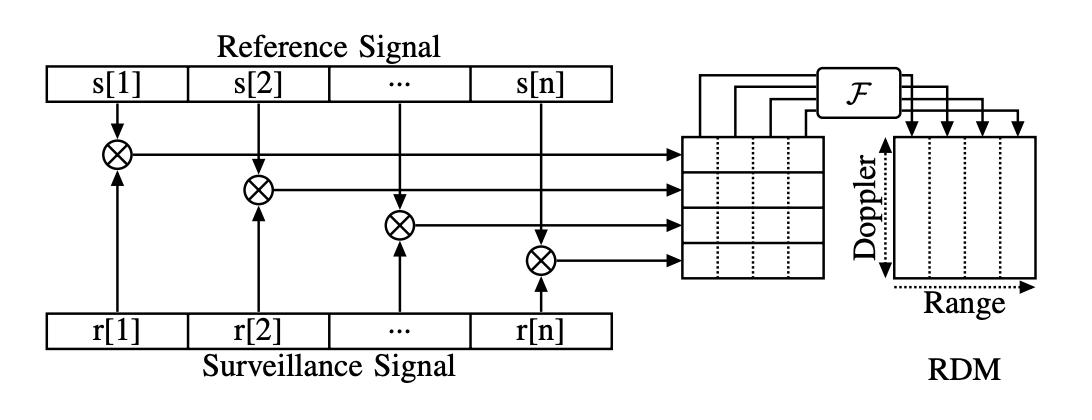
\includegraphics[width=0.8\textwidth]{FFT.png}
    \caption{Correlation and FFT for Range Doppler Mapping \cite{IOTpassiveRadar}}
    \label{fig:FFT}
\end{figure}

\todo[inline]{more general detail about the processing chain?}



\section{IoT Architecture}
\todo[inline]{keep section strictly about theory, not about specific hardware}

The IoT architecture in the scope of this project refers to the computational platforms utilised to undertake the digital signal processing which then maps to tracking and detection of the target. Existing studies have demonstrated the ability of off the shelf laptops \cite{FMlowCost}, and there is a few studies that use IoT platforms for FM signal processing \cite{IOTpassiveRadar}. The vital consideration when exploring hardware is the DSP requirements of the bistatic passive detection process (explored further in the next section).
\par \vspace{0.5cm} 
\noindent According to Schupbach et. al \cite{DABprocessingChain}, the broad scope capability requirements of the computational platform and associated processing can be grouped into signal acquisition, signal reconstruction and then the correlation function calculation. 
    
\noindent A possible IoT device that could be used, and has evidence of previous use as demonstrated by Moser et. al \cite{IOTpassiveRadar} is the Raspberry Pi platform, which despite having increased processing times, demonstrated its functionality. An alternate, higher powered choice in which Sednall demonstrated is the higher powered Nvidia Jetson, which includes faster processing times due to its quad core architecture \cite{FMlowCost}. The price for these options is \$60 compared to \$250 respectively. Ultimately, the choice of embedded IoT hardware for the project can be reduced to the trade off between low cost and processing power, and will be a key consideration in the project plan. Furthermore, there is possibility to design custom hardware to optimise for processing speeds and project cost, for example, a PCB extension utilising a Raspberry Pi with DSP IC chips and/or custom user buttons.

\section{Networking with Embedded Hardware}

Given that the overall goal of this thesis project is to create a low cost, embedded passive radar detection system, valuable to consider how this would be visualised, be it wired via ethernet / UART to PC or wireless protocol. 

\todo[inline]{add more about the theory of TCP/IP and networking over uq cloud, etc.}




% \begin{figure}[h]
%     \centering
%     
\includegraphics[width=0.25\textwidth]{UQLogo.png}
%     \caption{An Example Image}
%     \label{fig:uq}
% \end{figure}